%======================================================================
\chapter{Customized Reflector Array}
\label{ch: Chapter3}
%======================================================================

%----------------------------------------------------------------------
\section{Reflector Design}
%----------------------------------------------------------------------
The XBee RF modules that were used detect signals from any direction. For this project, however, it is desired to have differences in the received signals based on the angle from which the signal is coming. To accomplish this, two different models of reflector arrays were designed and constructed.

\subsection{Purely Paraboloidal Reflector}
The first design, shown in \autoref{fig:paraboloidalReflector}, uses a reflector with a purely paraboloidal shape. This shape was selected since all signals entering the reflector parallel to the axis of the reflector will pass through the focus of the paraboloid. By mounting the XBee such that the center of the antenna coincides with the focus of the paraboloid, the signal strength of the signals entering parallel to the axis will be maximized.
\begin{figure}
    \centering
    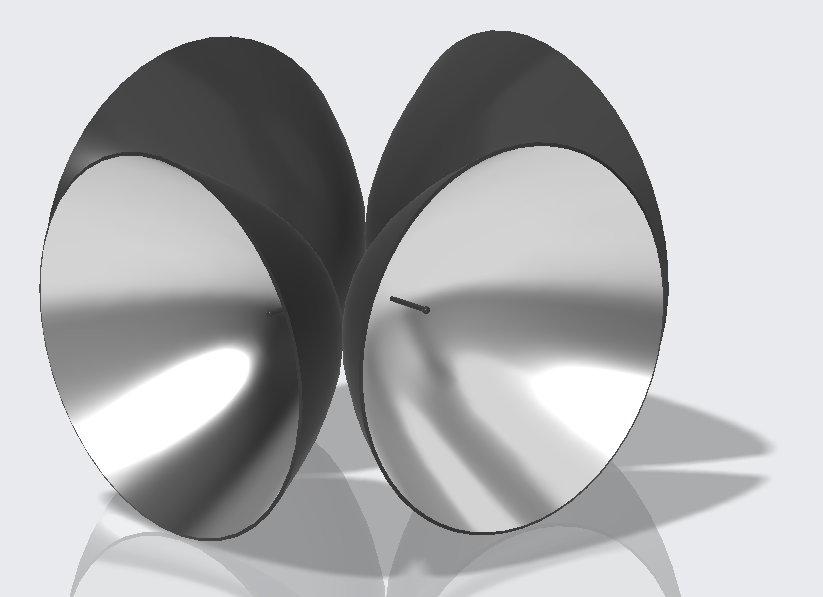
\includegraphics[width=3.5in]{figs/img/paraboloidalReflector.png}
    \caption{Purely Paraboloidal Reflector Array}
    \label{fig:paraboloidalReflector}
\end{figure}

\subsection{Combined Parabolic/Paraboloidal Reflector}
The second design, shown in \autoref{fig:parabolicReflector}, is the same on the lower half as the first design. However, the upper half is simply a surface where the horizontal cross-section is a parabola. The purpose for this design is similar to that of the first design, but the parabolic shape on the top will allow stronger detected signal strength of signals coming from above the reflector. Since the remote will be held by a person, it will generally be above the robot. The parabolic/paraboloidal reflector design is intended to allow better reception of signals from above.
\begin{figure}
    \centering
    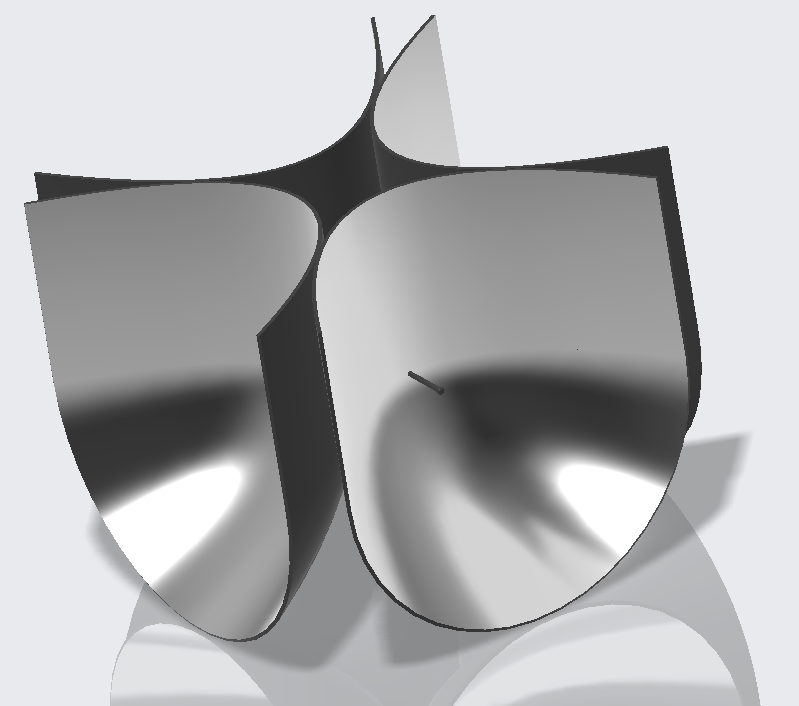
\includegraphics[width=3.5in]{figs/img/parabolicReflector.png}
    \caption{Parabolic/Paraboloidal Reflector Array}
    \label{fig:parabolicReflector}
\end{figure}

%----------------------------------------------------------------------
\section{Reflector Construction}
%----------------------------------------------------------------------
With the recent advancements in 3D printing technology, it is not difficult to create an object with a parabolic shape. In this project, the reflector dishes were created using a 3D printer. The reflector array was designed to be modular, where the dishes, top plate, and bottom frame were printed separately. After printing, the dishes were lined with foil tape to provide the reflective surface to focus the signals onto the antenna of the XBee. A layer of foil tape was also placed on the top plate to provide a ground plane for the XBee. The parts were then fastened together using M3 screws and nuts.

%----------------------------------------------------------------------
\section{Experimental Results}
%----------------------------------------------------------------------


%%% Local Variables:
%%% mode: latex
%%% TeX-master: "../finalReportMainV1"
%%% End: